\chapter{Apresentação e Análise de Resultados}

Breve descrição das próximas subseções...\\

Descrever a estratégia utilizada para ler os artigos. EX.: primeiro título, depois palavras-chave, resumo, conclusão, ...
Descrição das atividades realizadas na subseções...\\
Obs.: Inclua Figuras, Tabelas, Quadros, Códigos, etc...

\begin{figure}[htb]
	\caption{\label{fig:criterios}Fluxo de extração dos estudos}   
	\begin{center}
		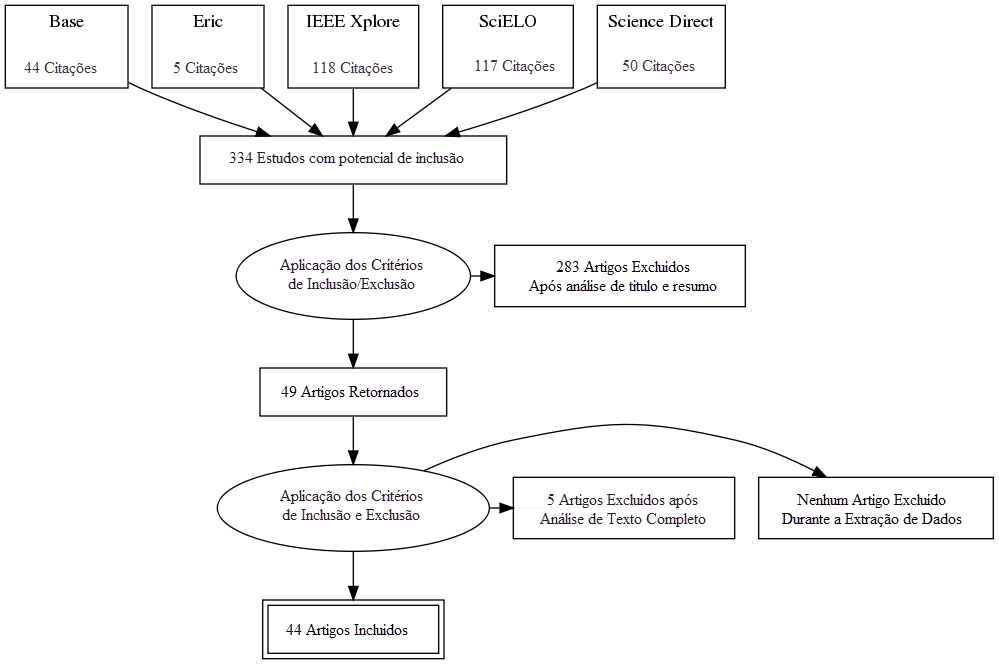
\includegraphics[scale=0.7]{Imagens/EstrategiadeBusca.dot.png}
	\end{center}
	\legend{Fonte: Elaborada pela autora}
\end{figure}

A Figura \ref{fig:criterios} apresenta um fluxo descrevendo o processo de extração dos artigos desde a base até a análise. Pode utilizar o site \url{http://prisma.thetacollaborative.ca/} para gerar automaticamente.

